\documentclass{article}
\usepackage[utf8]{inputenc}
\usepackage{tikz}
\usetikzlibrary{positioning}
\usetikzlibrary{shapes}

\begin{document}

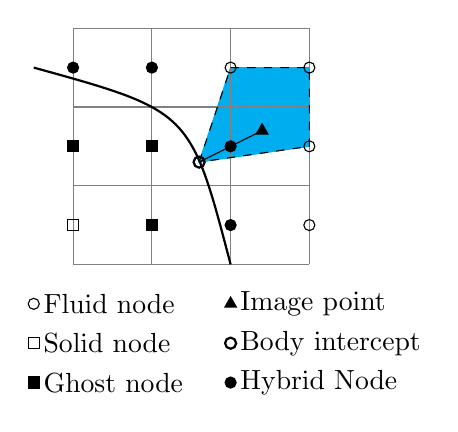
\begin{tikzpicture}
%stencil
%\filldraw[cyan] (0.5,0) rectangle (1.5,1);%shade
\filldraw[cyan] (0.1,-0.2) -- (0.5,1) -- (1.5,1) -- (1.5,0) -- cycle;
\draw [black, thick] (0.1,-0.2) circle (2pt);%BI
\node[fill=black,regular polygon, regular polygon sides=3,inner sep=1.0pt] at (0.9,0.2) {};%IP
\draw[black, thin] (0.1,-0.2) -- (0.9,0.2);%BIline

%grid
%horizontal
\draw[gray, thin] (-1.5,1.5) -- (1.5,1.5);
\draw[gray, thin] (-1.5,0.5) -- (1.5,0.5);
\draw[gray, thin] (-1.5,-0.5) -- (1.5,-0.5);
\draw[gray, thin] (-1.5,-1.5) -- (1.5,-1.5);
%vertical
\draw[gray, thin] (-1.5,1.5) -- (-1.5,-1.5);
\draw[gray, thin] (-0.5,1.5) -- (-0.5,-1.5);
\draw[gray, thin] (0.5,1.5) -- (0.5,-1.5);
\draw[gray, thin] (1.5,1.5) -- (1.5,-1.5);

%outline
\draw[black, thin, dashed] (0.1,-0.2) -- (0.5,1) -- (1.5,1) -- (1.5,0) -- cycle;
%fluid nodes
\draw [black] (0.5,1) circle (2pt);
\draw [black] (1.5,1) circle (2pt);
\draw [black] (1.5,0) circle (2pt);
\draw [black] (1.5,-1) circle (2pt);
%hybrid node
\filldraw [black] (-1.5,1) circle (2pt);
\filldraw [black] (-0.5,1) circle (2pt);
\filldraw [black] (0.5,0) circle (2pt);
\filldraw [black] (0.5,-1) circle (2pt);
%body
\draw[black, thick] (0.5,-1.5) .. controls (-0.01,0.45) .. (-2,1); 
%ghost nodes
\filldraw ([xshift=-2pt,yshift=-2pt]-1.5,0) rectangle ++(4pt,4pt);
\filldraw ([xshift=-2pt,yshift=-2pt]-0.5,0) rectangle ++(4pt,4pt);
\filldraw ([xshift=-2pt,yshift=-2pt]-0.5,-1) rectangle ++(4pt,4pt);
%solid node
\draw ([xshift=-2pt,yshift=-2pt]-1.5,-1) rectangle ++(4pt,4pt);
%legend
\draw [black] (-2.0,-2) circle (2pt); 
\node[anchor=west] at (-2.0,-2) {Fluid node};
\draw ([xshift=-2pt,yshift=-2pt]-2.0,-2.5) rectangle ++(4pt,4pt);
\node[anchor=west] at (-2.0,-2.5) {Solid node};
\filldraw ([xshift=-2pt,yshift=-2pt]-2.0,-3.0) rectangle ++(4pt,4pt);
\node[anchor=west] at (-2.0,-3.0) {Ghost node};


\filldraw [black] (0.5,-3.0) circle (2pt);
\node[anchor=west] at (0.5,-3.0) {Hybrid Node};
\draw [black, thick] (0.5,-2.5) circle (2pt);%BI
\node[anchor=west] at (0.5,-2.5) {Body intercept};
\node[fill=black,regular polygon, regular polygon sides=3,inner sep=1.0pt] at (0.5,-2.0) {};
\node[anchor=west] at (0.5,-2.0) {Image point};

\end{tikzpicture}


\end{document}
